\documentclass[11pt,a4paper]{article}
\usepackage[utf8]{inputenc}
\usepackage[T1]{fontenc}
\usepackage{lmodern}
\usepackage[margin=2.5cm]{geometry}
\usepackage{booktabs}
\usepackage{graphicx}
\usepackage{caption}
\usepackage{float}
\usepackage{amsmath}
\usepackage{breqn}
\usepackage[hidelinks]{hyperref}

\title{An automatic report for the dataset: 06-internet}
\author{Some Math empowered by some AI guided by some researchers}
\date{09 November 2026}

\begin{document}
\maketitle

\noindent\emph{Produced by \texttt{autostat}, a Python 3 port of the Automatic Bayesian Covariance Discovery system of Lloyd et al. (AAAI 2014).}


\begin{figure}[H]
\centering
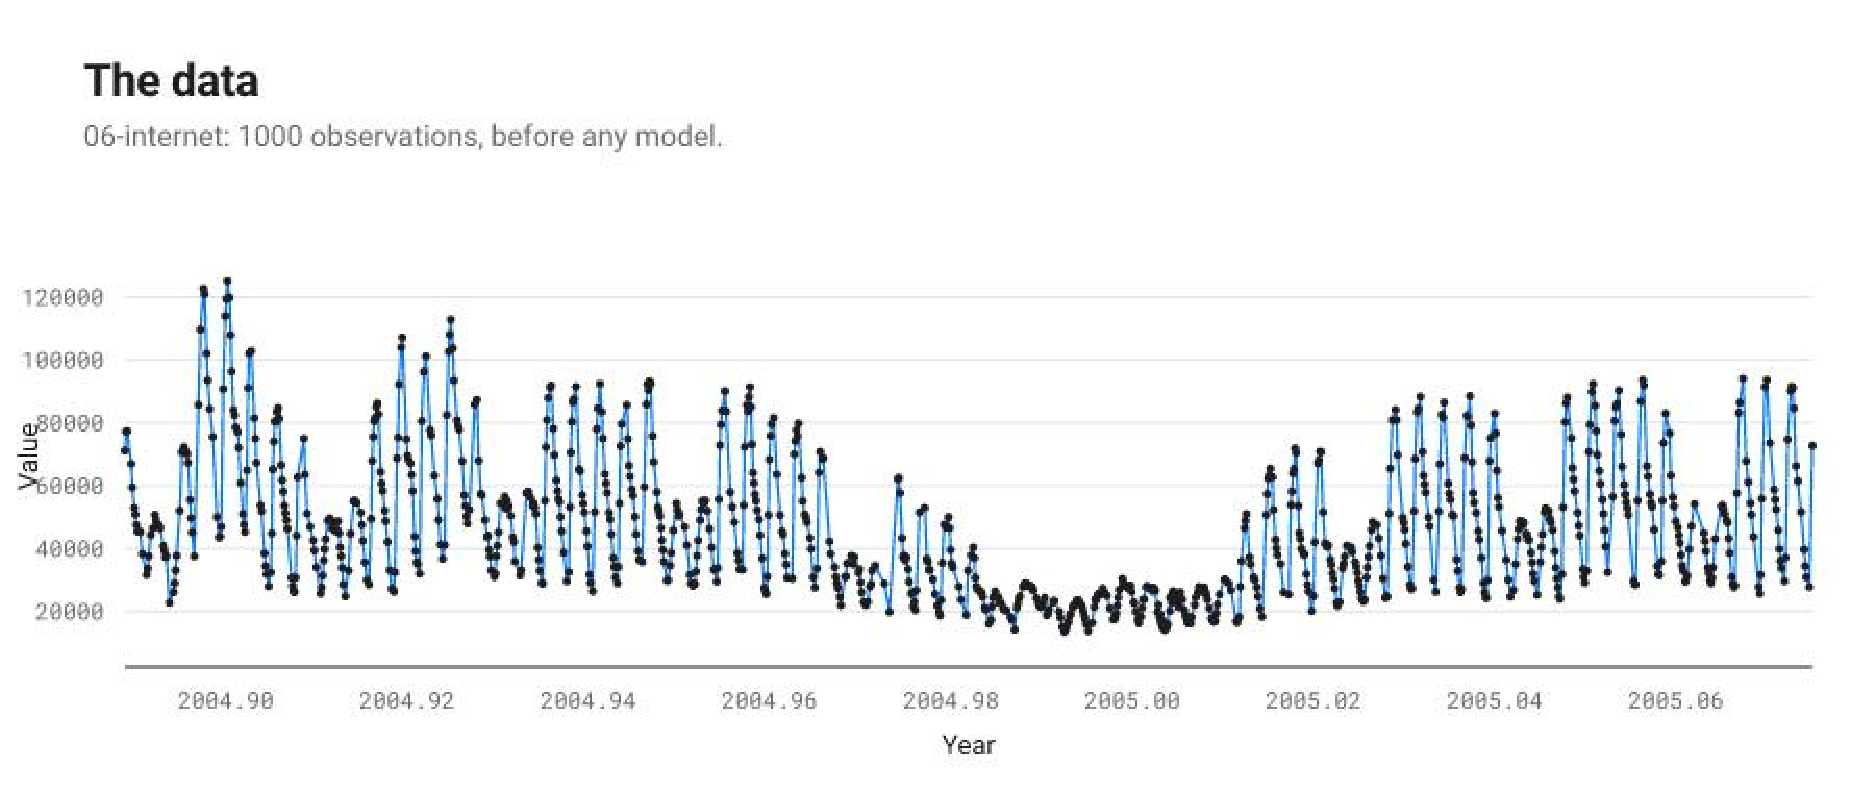
\includegraphics[width=\linewidth]{data.pdf}
\caption*{The data}
\end{figure}

\section*{Executive summary}

The structure search selected \texttt{CW(WN + Per x SE + Per x SE + SE, SE) + C + WN} (Bayesian information criterion 19323.2; negative log likelihood 9599.4 on 1000 points). It decomposes into 7 additive components, listed by how much each reduces extrapolation error:
\begin{enumerate}
  \item A constant.
  \item A very smooth function. This function applies from 14 Dec 2004 until 28 Dec 2004.
  \item An approximately periodic function with a period of 24.0 hours. This function applies until 14 Dec 2004 and from 28 Dec 2004 onwards.
  \item A very approximately periodic function with a period of 3.9 days. This function applies until 14 Dec 2004 and from 28 Dec 2004 onwards.
  \item A smooth function. This function applies until 14 Dec 2004 and from 28 Dec 2004 onwards.
  \item Uncorrelated noise. This function applies until 14 Dec 2004 and from 28 Dec 2004 onwards.
  \item Uncorrelated noise.
\end{enumerate}

\begin{center}
\begin{tabular}{lrrrr}
\toprule
\# & $R^2$ cumulative (\%) & Residual variance explained (\%) & CV MAE & MAE reduction (\%) \\
\midrule
data & & & 4.64e+04 & \\
1 & 0.0 & 0.0 & 2.04e+04 & 56.0 \\
2 & 32.4 & 32.4 & 1.39e+04 & 31.9 \\
3 & 72.6 & 59.5 & 7.88e+03 & 43.2 \\
4 & 99.6 & 98.7 & 7.73e+03 & 1.9 \\
5 & 99.6 & 0.0 & 7.73e+03 & 0.0 \\
6 & 99.9 & 70.4 & 7.73e+03 & 0.0 \\
7 & 100.0 & 100.0 & 7.73e+03 & 0.0 \\
\bottomrule
\end{tabular}
\end{center}

MAE: mean absolute error over ten contiguous held-out blocks; CV: cross-validated.

\section*{The formula found}

The structure search is a symbolic regression: it searches a grammar of expressions over kernels and keeps the one with the lowest Bayesian information criterion. This is the expression it kept, with every fitted parameter in place; $t$ is in years.
\begin{dmath*}
y(t) = f_{1}(t) + f_{2}(t) + f_{3}(t) + f_{4}(t) + f_{5}(t) + f_{6}(t) + f_{7}(t)
\end{dmath*}

Each component is a Gaussian process with its own covariance:
\begin{dmath*}
f_{1}(t) \sim \mathrm{GP}\!\left(0,\ 8.171 \times 10^{9}\right)
\end{dmath*}
\begin{dmath*}
f_{2}(t) \sim \mathrm{GP}\!\left(0,\ w_{1}(t)\,w_{1}(t')\left[8.054 \times 10^{8}\,\exp\!\left(-\frac{(t - t')^2}{2 \cdot 0.2725^2}\right)\right]\right)
\end{dmath*}
\begin{dmath*}
f_{3}(t) \sim \mathrm{GP}\!\left(0,\ (1 - w_{1}(t))(1 - w_{1}(t'))\left[1.69 \times 10^{8}\,\frac{\exp\!\left(3.234\cos\frac{2\pi (t - t')}{0.002739}\right) - I_0(3.234)}{e^{3.234} - I_0(3.234)} \cdot \exp\!\left(-\frac{(t - t')^2}{2 \cdot 1.03^2}\right)\right]\right)
\end{dmath*}
\begin{dmath*}
f_{4}(t) \sim \mathrm{GP}\!\left(0,\ (1 - w_{1}(t))(1 - w_{1}(t'))\left[1.896 \times 10^{8}\,\frac{\exp\!\left(1.149\cos\frac{2\pi (t - t')}{0.01064}\right) - I_0(1.149)}{e^{1.149} - I_0(1.149)} \cdot \exp\!\left(-\frac{(t - t')^2}{2 \cdot \left(5.787 \times 10^{-4}\right)^2}\right)\right]\right)
\end{dmath*}
\begin{dmath*}
f_{5}(t) \sim \mathrm{GP}\!\left(0,\ (1 - w_{1}(t))(1 - w_{1}(t'))\left[56384\,\exp\!\left(-\frac{(t - t')^2}{2 \cdot 0.02954^2}\right)\right]\right)
\end{dmath*}
\begin{dmath*}
f_{6}(t) \sim \mathrm{GP}\!\left(0,\ (1 - w_{1}(t))(1 - w_{1}(t'))\left[2.163 \times 10^{6}\,\delta_{t t'}\right]\right)
\end{dmath*}
\begin{dmath*}
f_{7}(t) \sim \mathrm{GP}\!\left(0,\ 1.682 \times 10^{6}\,\delta_{t t'}\right)
\end{dmath*}

The changes of regime weigh the components with:
\begin{dmath*}
w_{1}(t) = \tfrac{1}{4}\left(1 + \tanh\left(60.58\,(t - 2005)\right)\right)\left(1 - \tanh\left(60.58\,(t - 2005)\right)\right)
\end{dmath*}

These components have a closed form, read from their posterior mean:
\begin{dmath*}
f_{1}(t) = 55049
\end{dmath*}

The other components are smooth, quasi-periodic or noise without a short formula: a draw from such a process has no finite closed form; its covariance above is the formula.

Closed form of each component:

\begin{center}\footnotesize
\begin{tabular}{lp{0.36\linewidth}l}
\toprule
\# & component & closed form \\
\midrule
1 & A constant & exact polynomial of degree 0 \\
2 & A very smooth function. This function applies from 14 Dec 2004 until 28 Dec 2004 & none: the covariance is the formula \\
3 & An approximately periodic function with a period of 24.0 hours. This function applies until 14 Dec 2004 and from 28 Dec 2004 onwards & none: the covariance is the formula \\
4 & A very approximately periodic function with a period of 3.9 days. This function applies until 14 Dec 2004 and from 28 Dec 2004 onwards & none: the covariance is the formula \\
5 & A smooth function. This function applies until 14 Dec 2004 and from 28 Dec 2004 onwards & none: the covariance is the formula \\
6 & Uncorrelated noise. This function applies until 14 Dec 2004 and from 28 Dec 2004 onwards & none: the covariance is the formula \\
7 & Uncorrelated noise & none: the covariance is the formula \\
\bottomrule
\end{tabular}
\end{center}

\section*{Search path and stopping criterion}

The 2014 configuration searches a fixed number of levels and keeps the lowest BIC; it has no stopping rule. The table follows the winner of each level. A change of structure adds or removes terms; a level that keeps the structure only refits its parameters. BIC differences read on the scale of Kass and Raftery (1995): under 2 barely worth mentioning, 2 to 6 positive, 6 to 10 strong, over 10 very strong.

\begin{center}\footnotesize
\begin{tabular}{lllp{0.36\linewidth}lll}
\toprule
level & BIC & change & structure & components & closed & params \\
\midrule
1 & 22392.0 &  & WN + SE & 2 & 0 & 3 \\
2 & 20259.3 & -2132.7 & WN + Per x SE + SE & 3 & 0 & 7 \\
3 & 19605.9 & -653.4 & WN + Per x SE + Per x SE + SE + SE & 5 & 0 & 13 \\
4 & 19374.7 & -231.2 & CW(Per x SE + Per x SE + SE, C) + WN + SE & 6 & 1 & 17 \\
5 & 19373.0 & -1.7 & CW(Per x SE + Per x SE + SE, C) + WN + SE & 6 & 1 & 17 \\
6 & 19352.3 & -20.7 & CW(Per x SE + Per x SE + SE, C) + WN + SE & 6 & 1 & 17 \\
7 & 19352.3 & +0.0 & CW(Per x SE + Per x SE + SE, C) + WN + SE & 6 & 1 & 17 \\
8 & 19352.3 & +0.0 & CW(Per x SE + Per x SE + SE, C) + WN + SE & 6 & 1 & 17 \\
9 & 19349.4 & -2.9 & CW(Per x SE + Per x SE + SE, SE) + C + WN & 6 & 1 & 17 \\
10 (kept) & 19323.2 & -26.3 & CW(WN + Per x SE + Per x SE + SE, SE) + C + WN & 7 & 1 & 18 \\
\bottomrule
\end{tabular}
\end{center}

\begin{figure}[H]
\centering
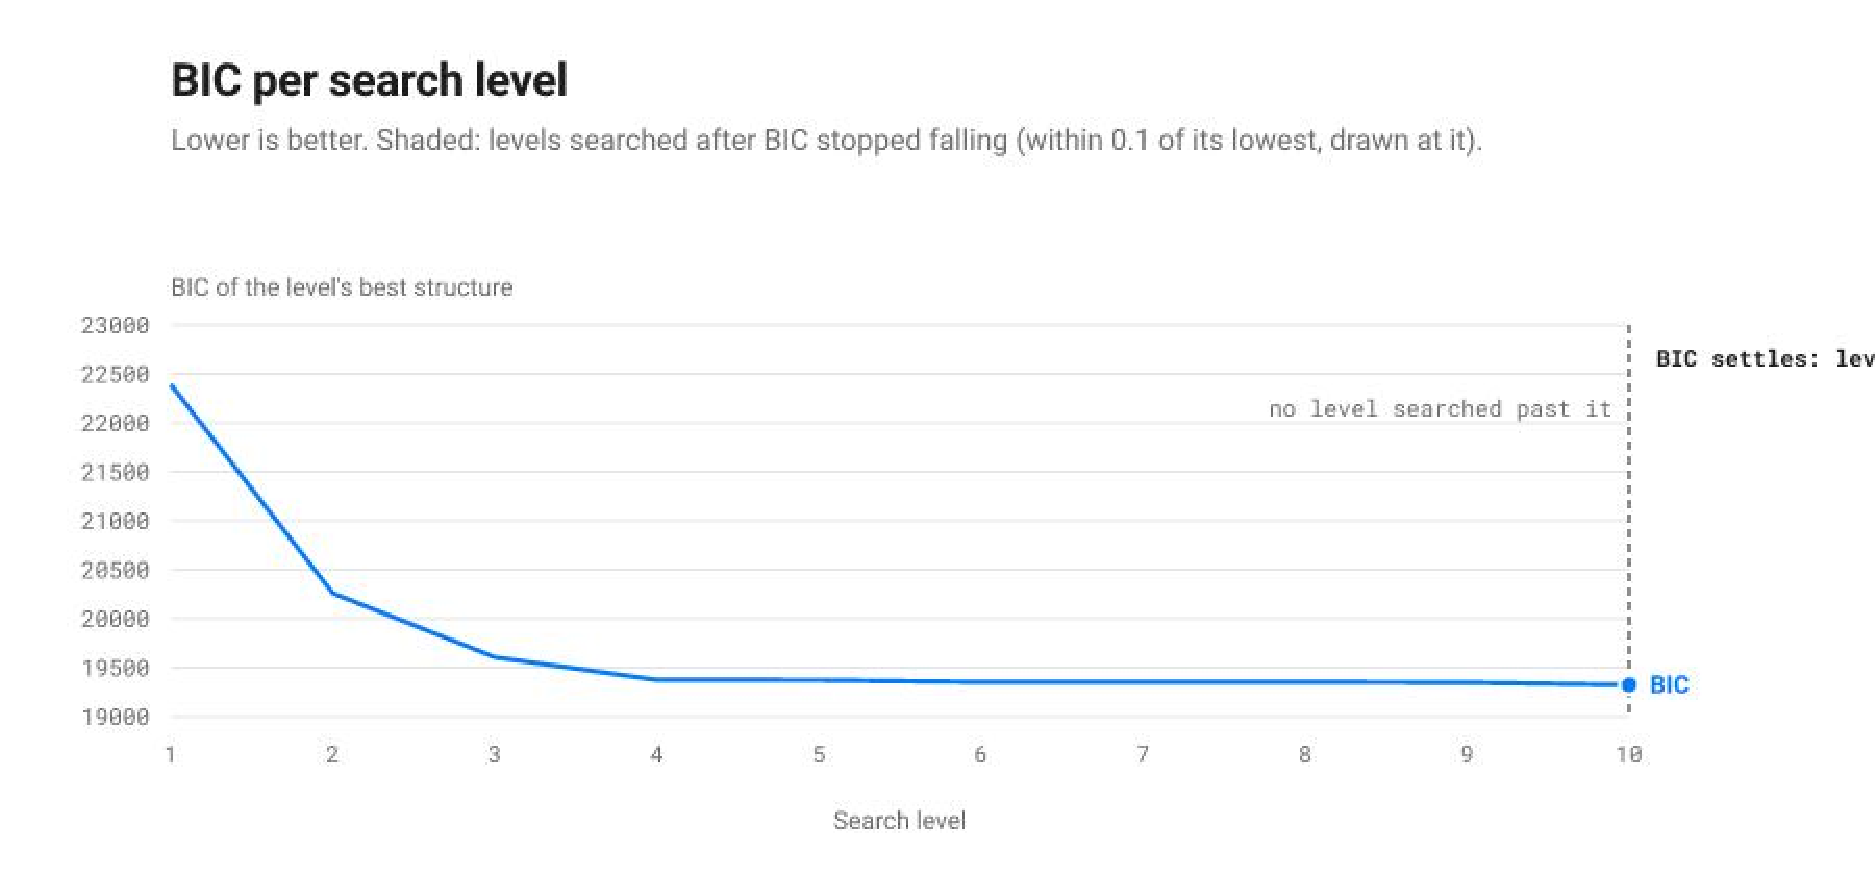
\includegraphics[width=\linewidth]{bic.pdf}
\caption*{BIC per search level}
\end{figure}

Posterior weight of each structure met, exp(-BIC/2) normalised under a flat prior, after the Bayesian machine scientist (Guimerà et al., 2020): where the search keeps one structure, the weights say how much the data prefer it to the others. The 5 structure(s) under 0.001 are left out.

\begin{center}\footnotesize
\begin{tabular}{p{0.36\linewidth}ll}
\toprule
structure & lowest BIC & weight \\
\midrule
CW(WN + Per x SE + Per x SE + SE, SE) + C + WN & 19323.2 & 1.000 \\
\bottomrule
\end{tabular}
\end{center}

\begin{itemize}
\item The search ran 10 levels (the published 2014 search: ten levels, no stopping rule) and keeps the model of level 10, CW(WN + Per x SE + Per x SE + SE, SE) + C + WN, BIC 19323.2.
\item The best different structure, CW(Per x SE + Per x SE + SE, SE) + C + WN (level 9), is 26.3 above it: very strong evidence for the kept one on the Kass and Raftery scale.
\item Weighed by exp(-BIC/2) under a flat prior, as the Bayesian machine scientist weighs expressions, the structures met give the kept one a posterior weight of 1.000 and the next, CW(Per x SE + Per x SE + SE, SE) + C + WN, 0.000: the kept one takes almost all the weight.
\item The last level still changed the structure and lowered BIC by 26.3: more levels might find a better expression.
\item A rule stopping after 1 level(s) without a fall above 0.1 would have ended the search at level 7 and kept CW(Per x SE + Per x SE + SE, C) + WN + SE (level 6, BIC 29.2 above).
\item A rule stopping after 2 level(s) without a fall above 0.1 would have ended the search at level 8 and kept CW(Per x SE + Per x SE + SE, C) + WN + SE (level 6, BIC 29.2 above).
\item The kept expression has 18 parameters for 1000 points: its BIC is a fit term 2 NLL = 19198.8 plus a complexity term p ln n = 124.3, each extra parameter costing 6.91; it splits into 7 components, 1 of them with a closed form.
\end{itemize}

\begin{figure}[H]
\centering
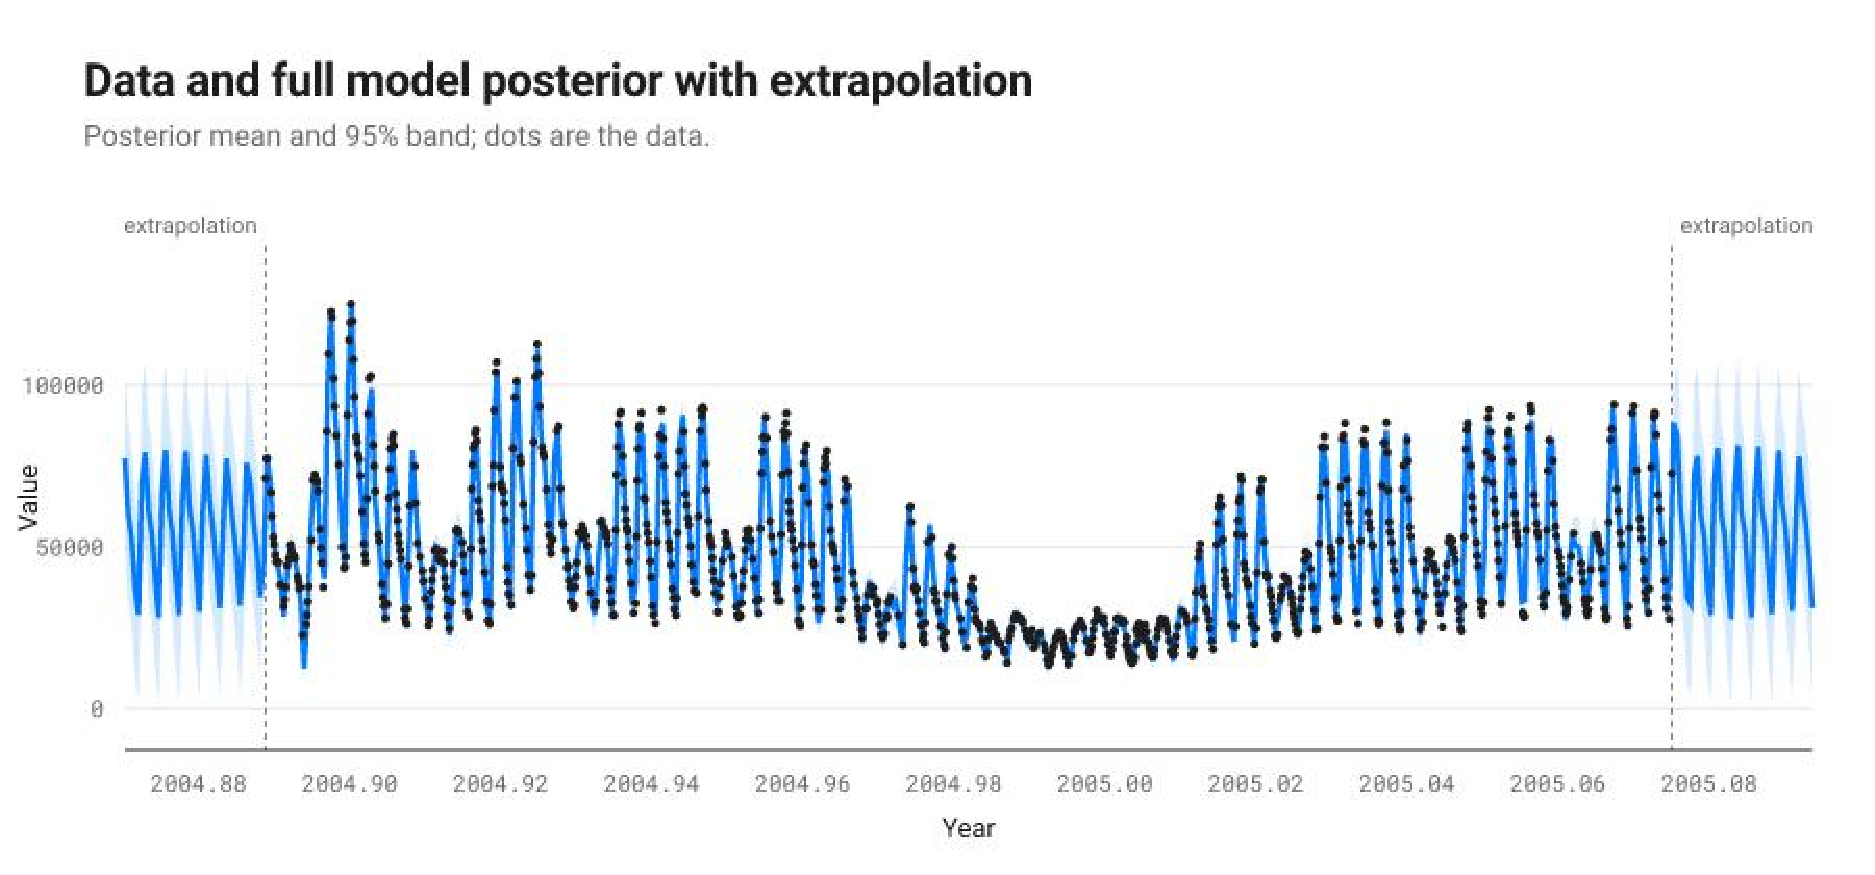
\includegraphics[width=\linewidth]{fit.pdf}
\caption*{Data and full posterior}
\end{figure}

\section*{Detailed discussion of the components}

\subsection*{Component 1: A constant}

This component is constant.

This component explains 0.0\% of the data's variance on its own; with the components above it, 0.0\%. Adding it changes the cross-validated MAE by -56.0\%.

\emph{Extrapolation.} This component is assumed to stay constant.

\begin{figure}[H]
\centering
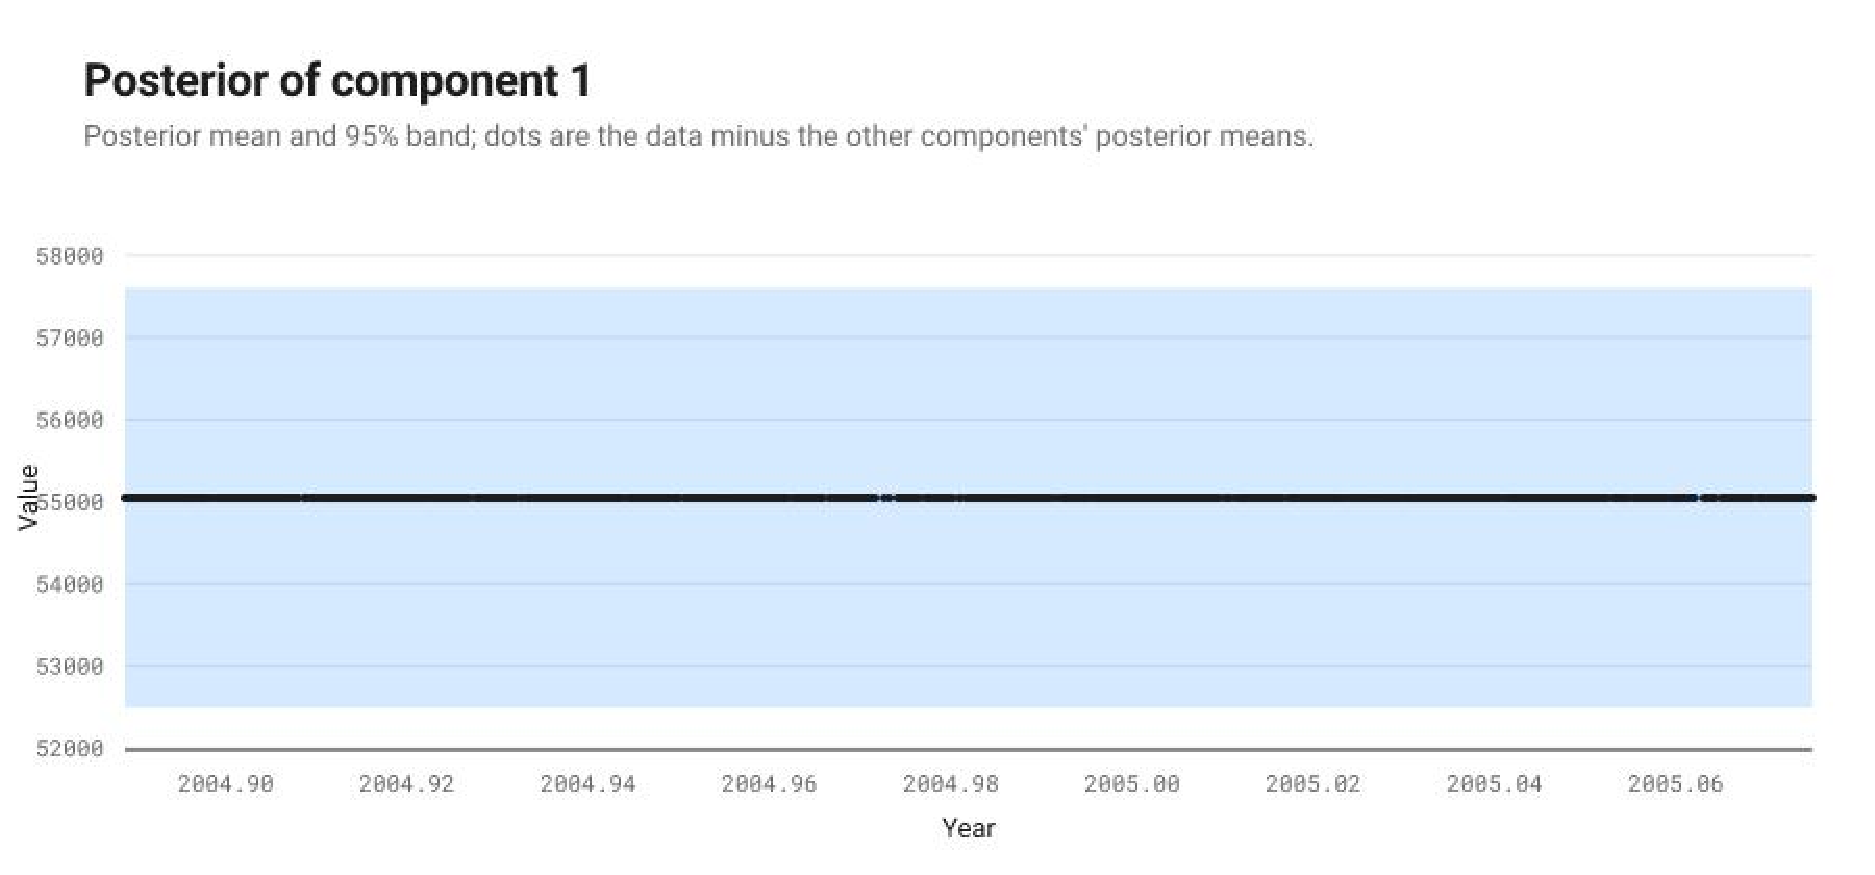
\includegraphics[width=\linewidth]{component_1.pdf}
\caption*{Component 1}
\end{figure}
\subsection*{Component 2: A very smooth function. This function applies from 14 Dec 2004 until 28 Dec 2004}

This component is a very smooth function. This component applies from 14 Dec 2004 until 28 Dec 2004.

This component explains 32.4\% of the data's variance on its own; with the components above it, 32.4\%. Adding it changes the cross-validated MAE by -31.9\%.

\emph{Extrapolation.} This component is assumed to stop before the end of the data and will therefore be extrapolated as zero.

\begin{figure}[H]
\centering
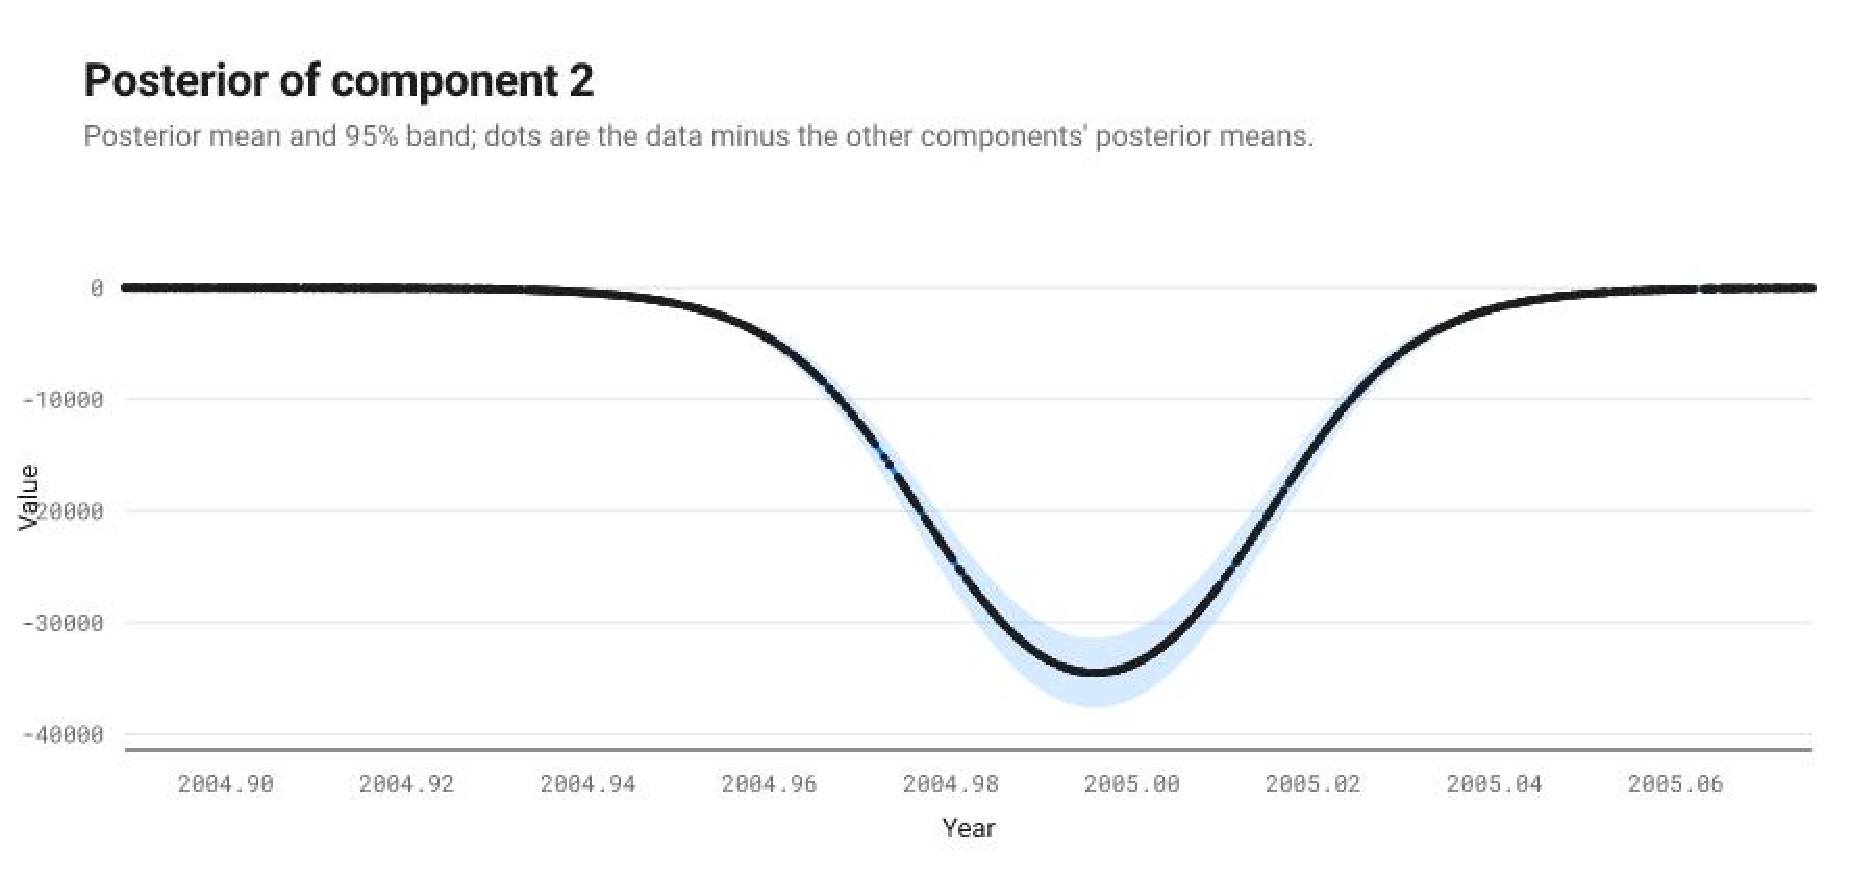
\includegraphics[width=\linewidth]{component_2.pdf}
\caption*{Component 2}
\end{figure}
\subsection*{Component 3: An approximately periodic function with a period of 24.0 hours. This function applies until 14 Dec 2004 and from 28 Dec 2004 onwards}

This component is approximately periodic with a period of 24.0 hours. Across periods the shape of this function varies very smoothly. The shape of this function within each period has a typical lengthscale of 2.1 hours. This component applies until 14 Dec 2004 and from 28 Dec 2004 onwards.

This component explains 39.3\% of the data's variance on its own; with the components above it, 72.6\%. Adding it changes the cross-validated MAE by -43.2\%.

\emph{Extrapolation.} This component is assumed to continue to be approximately periodic. The shape of the function is assumed to vary very smoothly between periods but will eventually return to the prior. The prior is entirely uncertain about the phase of the periodic function. Consequently the pointwise posterior will appear to lose its periodicity, but this merely reflects the uncertainty in the shape and phase of the function.

\begin{figure}[H]
\centering
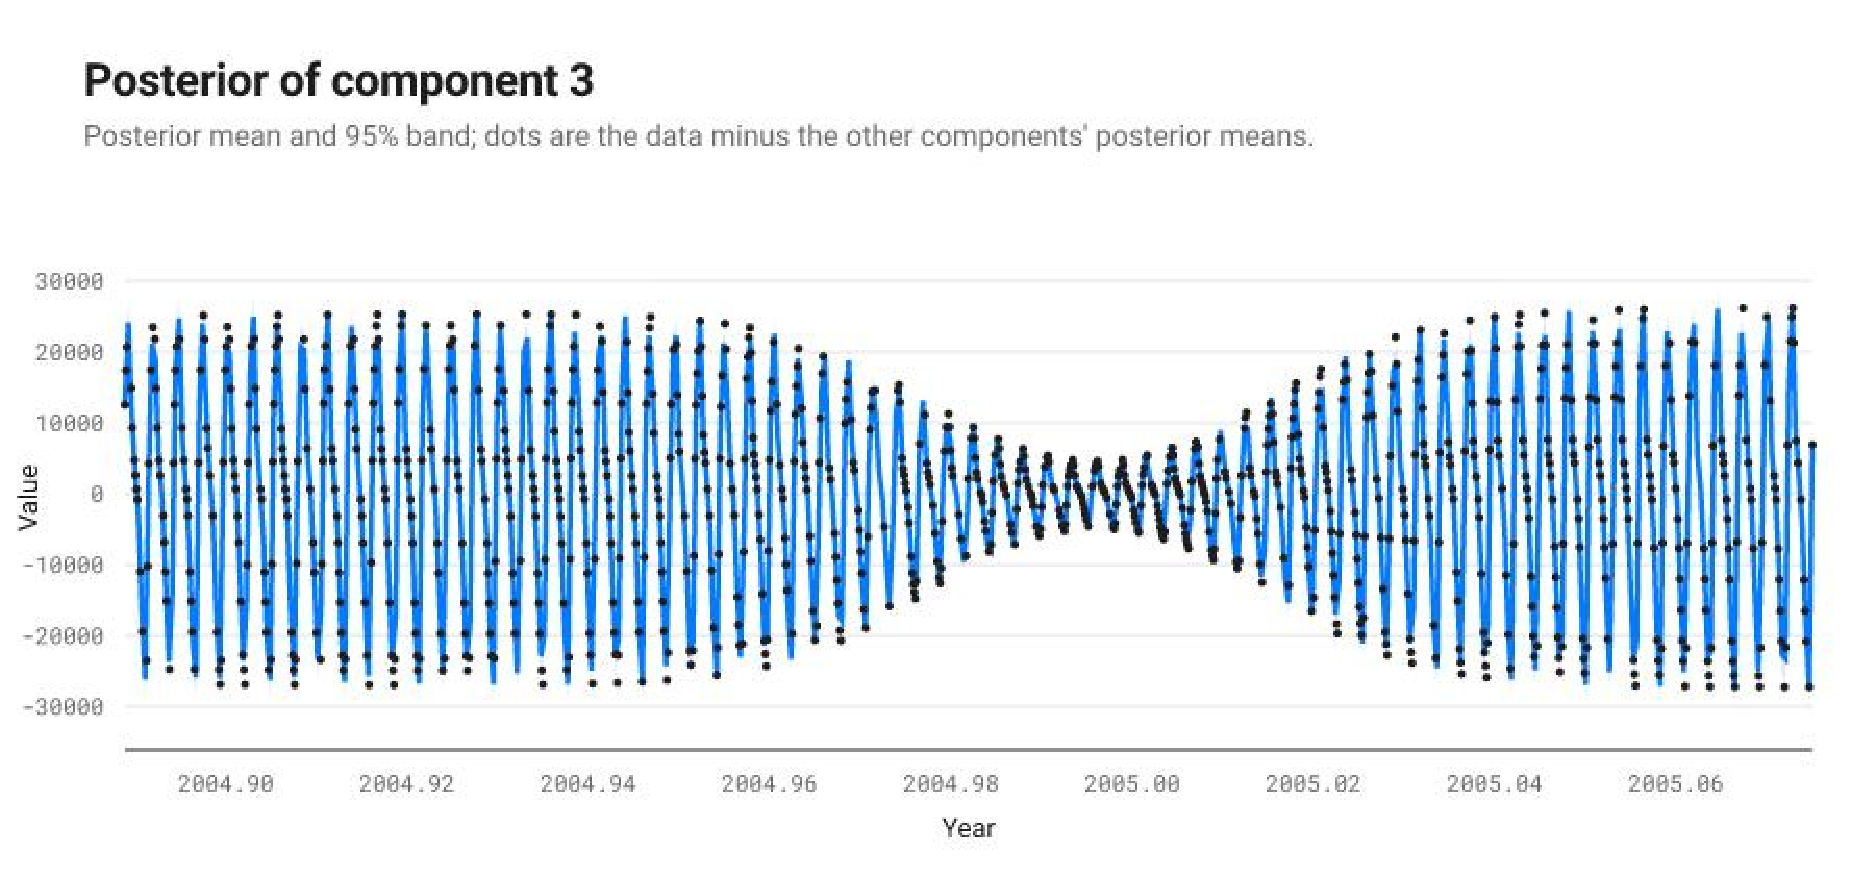
\includegraphics[width=\linewidth]{component_3.pdf}
\caption*{Component 3}
\end{figure}
\subsection*{Component 4: A very approximately periodic function with a period of 3.9 days. This function applies until 14 Dec 2004 and from 28 Dec 2004 onwards}

This component is very approximately periodic with a period of 3.9 days. Across periods the shape of this function varies smoothly with a typical lengthscale of 5.1 hours. Since this lengthscale is small relative to the period this component may more closely resemble a non-periodic smooth function. This component applies until 14 Dec 2004 and from 28 Dec 2004 onwards.

This component explains 33.3\% of the data's variance on its own; with the components above it, 99.6\%. Adding it changes the cross-validated MAE by -1.9\%.

\emph{Extrapolation.} This component is assumed to continue to be approximately periodic. The shape of the function is assumed to vary smoothly between periods but will quickly return to the prior. The prior is entirely uncertain about the phase of the periodic function. Consequently the pointwise posterior will appear to lose its periodicity, but this merely reflects the uncertainty in the shape and phase of the function.

\begin{figure}[H]
\centering
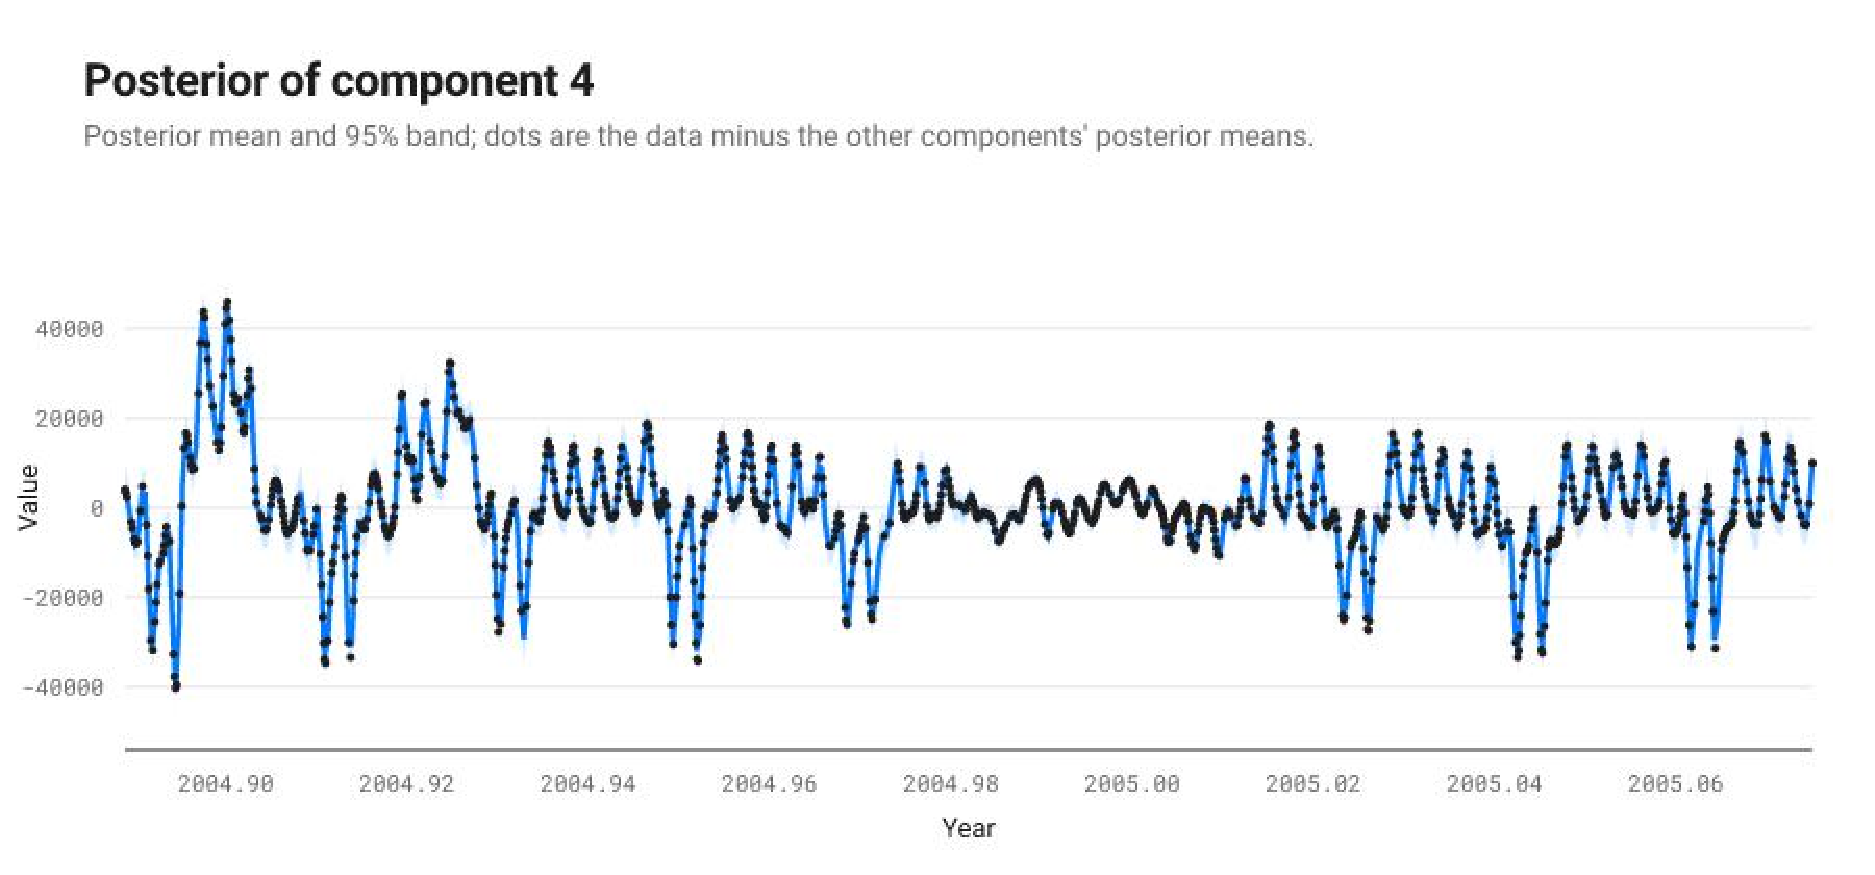
\includegraphics[width=\linewidth]{component_4.pdf}
\caption*{Component 4}
\end{figure}
\subsection*{Component 5: A smooth function. This function applies until 14 Dec 2004 and from 28 Dec 2004 onwards}

This component is a smooth function with a typical lengthscale of 10.8 days. This component applies until 14 Dec 2004 and from 28 Dec 2004 onwards.

This component explains 0.0\% of the data's variance on its own; with the components above it, 99.6\%. Adding it changes the cross-validated MAE by -0.0\%.

\emph{Extrapolation.} This component is assumed to continue smoothly but is also assumed to be stationary so its distribution will return to the prior. The prior distribution places mass on smooth functions with a marginal mean of zero and a typical lengthscale of 10.8 days.

\begin{figure}[H]
\centering
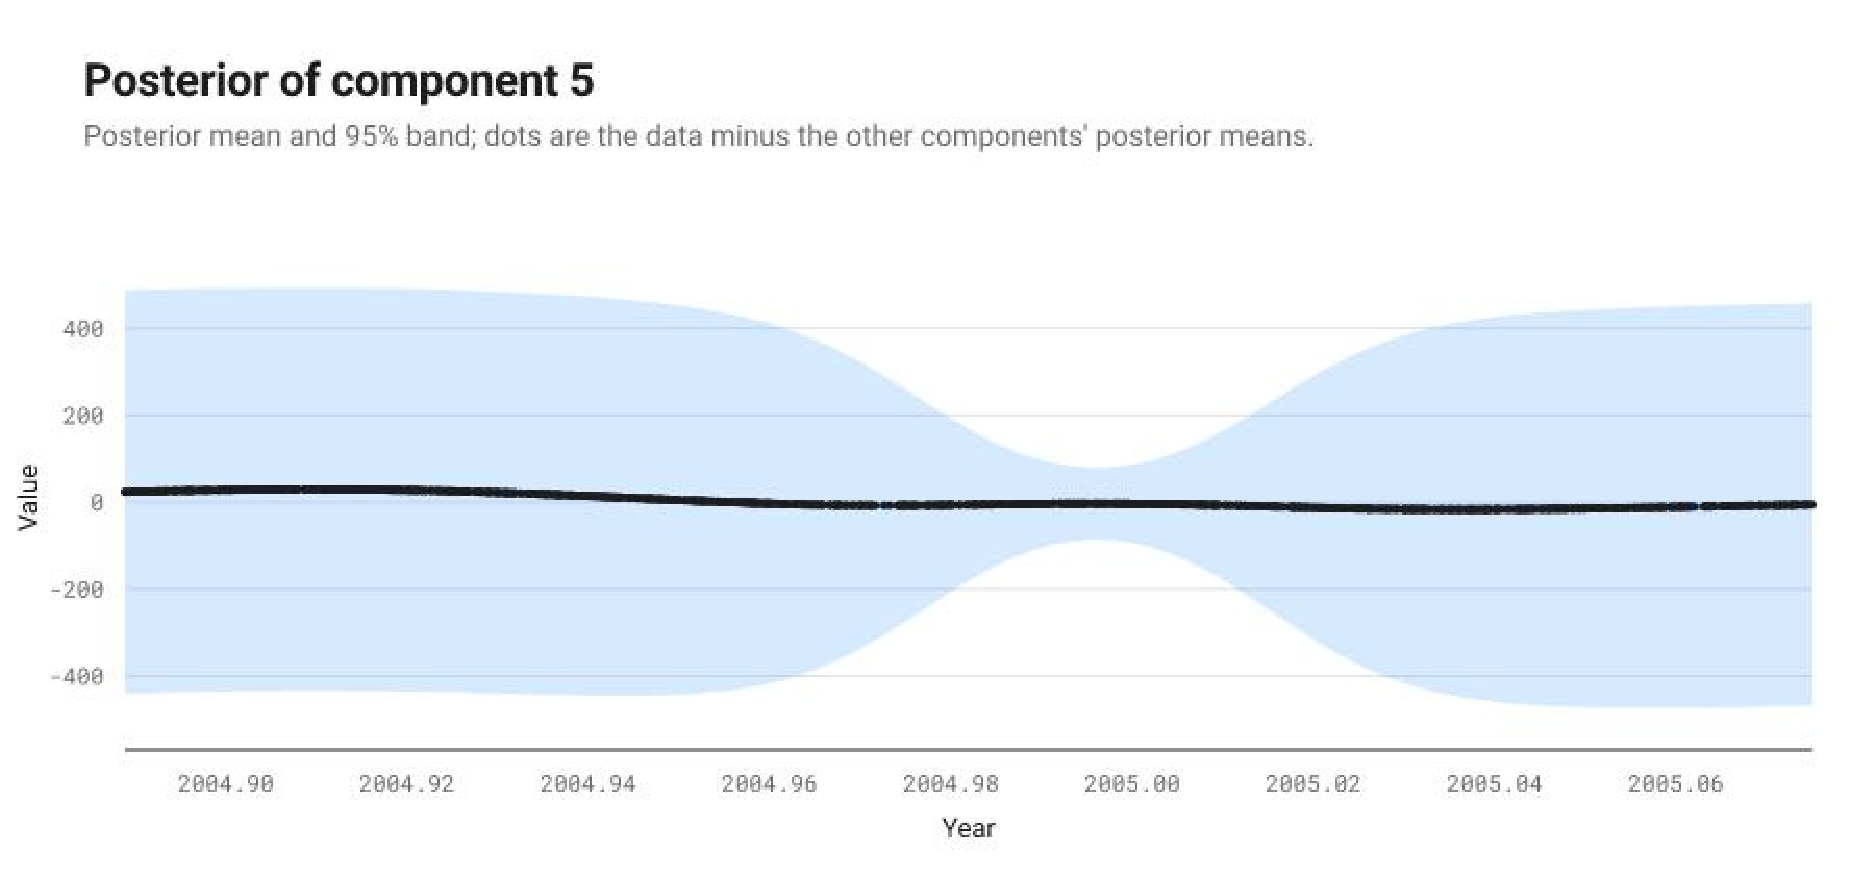
\includegraphics[width=\linewidth]{component_5.pdf}
\caption*{Component 5}
\end{figure}
\subsection*{Component 6: Uncorrelated noise. This function applies until 14 Dec 2004 and from 28 Dec 2004 onwards}

This component models uncorrelated noise. This component applies until 14 Dec 2004 and from 28 Dec 2004 onwards.

This component explains 0.5\% of the data's variance on its own; with the components above it, 99.9\%. Adding it changes the cross-validated MAE by -0.0\%.

\emph{Extrapolation.} This component assumes the uncorrelated noise will continue indefinitely.

\begin{figure}[H]
\centering
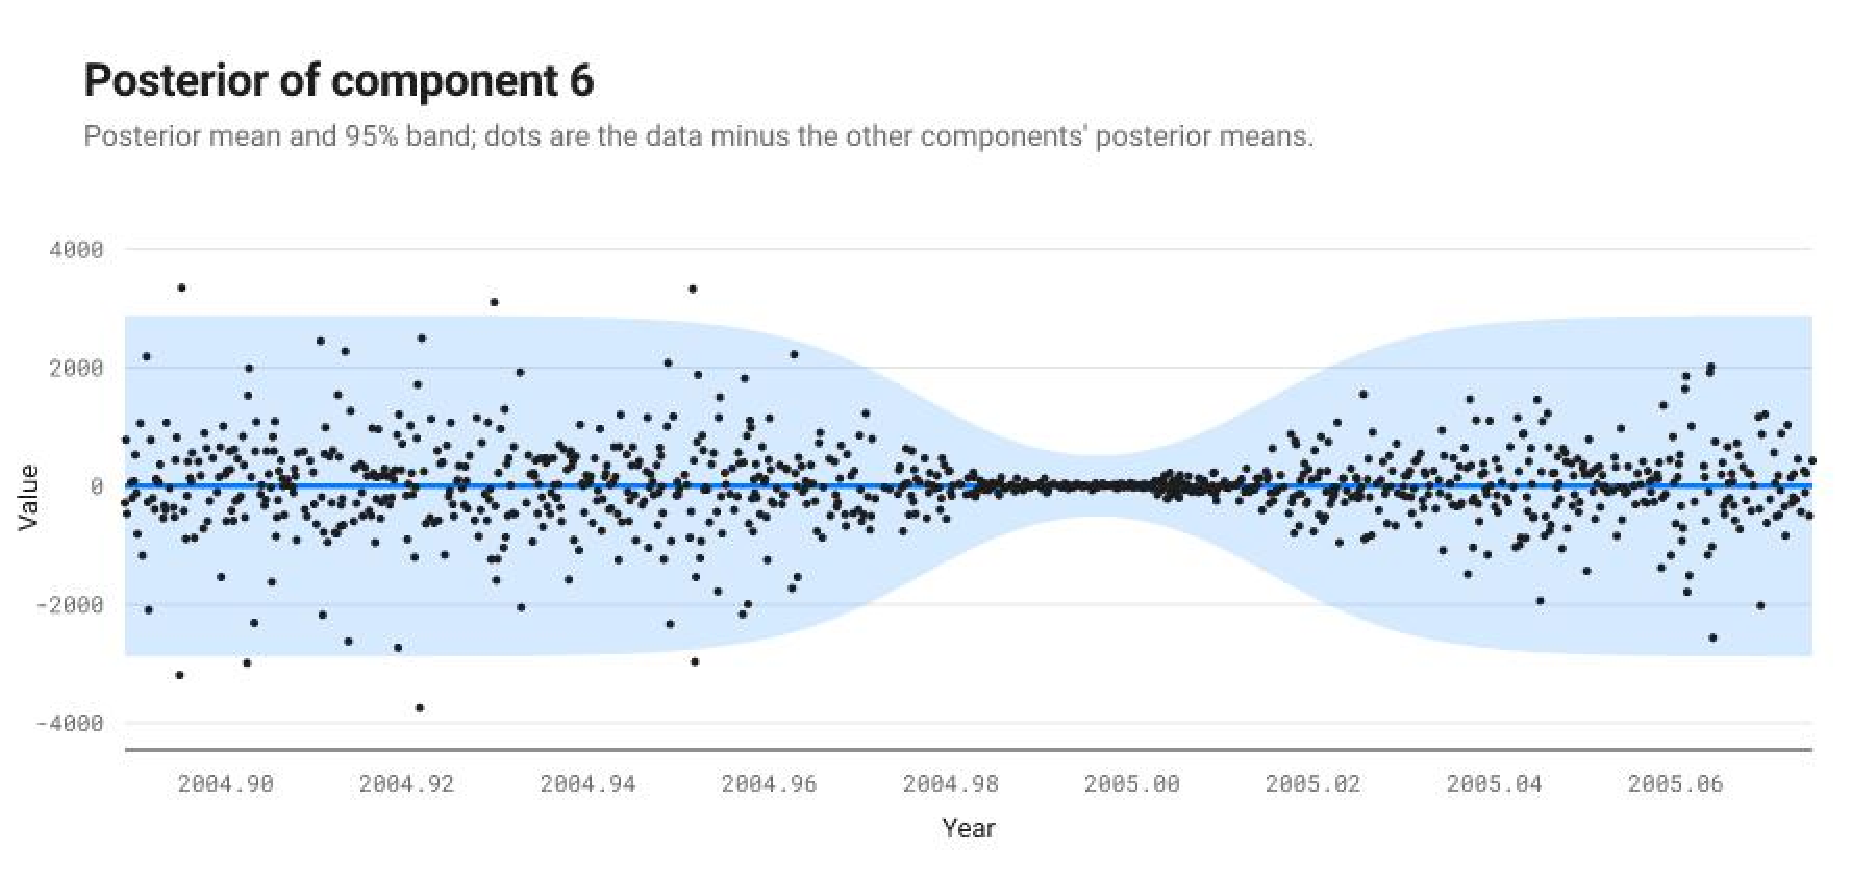
\includegraphics[width=\linewidth]{component_6.pdf}
\caption*{Component 6}
\end{figure}
\subsection*{Component 7: Uncorrelated noise}

This component models uncorrelated noise.

This component explains 0.5\% of the data's variance on its own; with the components above it, 100.0\%. Adding it changes the cross-validated MAE by -0.0\%.

\emph{Extrapolation.} This component assumes the uncorrelated noise will continue indefinitely.

\begin{figure}[H]
\centering
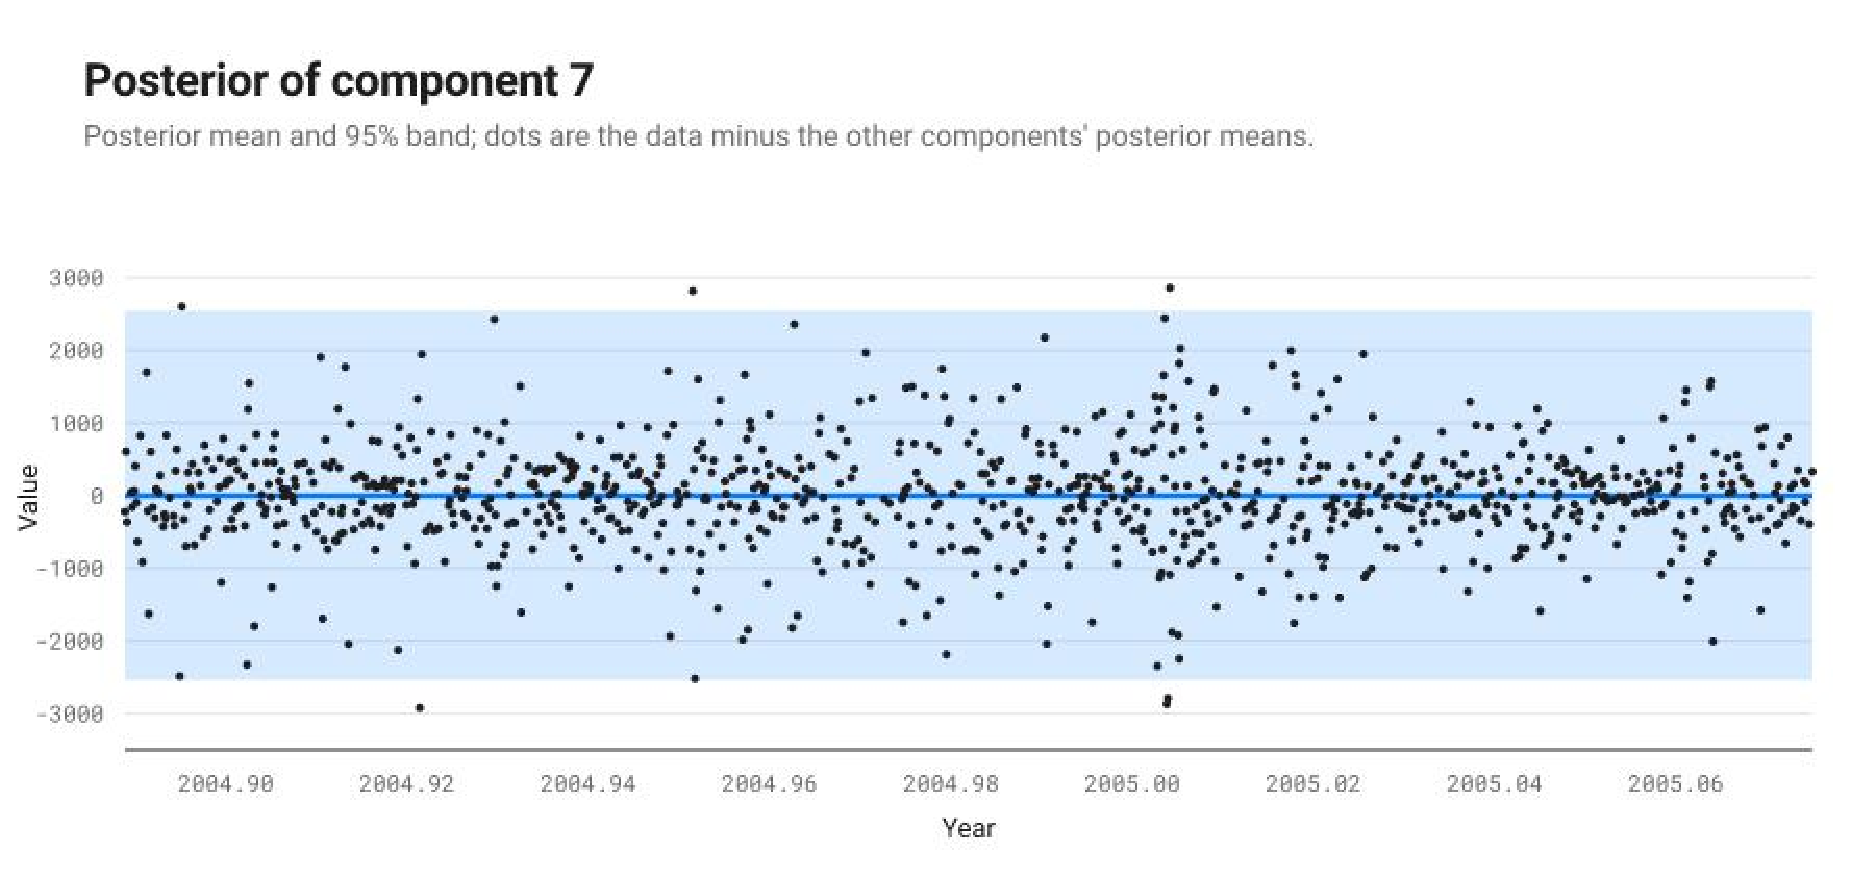
\includegraphics[width=\linewidth]{component_7.pdf}
\caption*{Component 7}
\end{figure}

\section*{Model checking}

Each statistic compares draws of a component's posterior with draws of its prior. A small p-value (bold below 0.05) points at a property of the data that the component's prior does not reproduce.

\begin{center}
\begin{tabular}{lrrrrrrr}
\toprule
\# & QQ max & QQ min & ACF min & ACF min lag & Pgram max & Pgram peak & MMD \\
\midrule
1 & 0.538 & 0.538 & 0.680 & 0.512 & 0.966 & 0.968 & \textbf{0.000} \\
2 & 0.128 & 0.378 & 0.804 & 0.788 & 0.254 & 0.980 & \textbf{0.000} \\
3 & 0.356 & 0.492 & 0.626 & 0.748 & 0.164 & 0.578 & \textbf{0.000} \\
4 & 0.278 & 0.962 & \textbf{0.000} & 0.480 & \textbf{0.000} & 0.522 & \textbf{0.000} \\
5 & 0.924 & 0.958 & 0.986 & 0.970 & 0.950 & 1.000 & 0.311 \\
6 & 0.788 & 0.608 & 0.960 & 0.984 & 0.968 & 0.948 & \textbf{0.000} \\
7 & 0.894 & 0.860 & 0.972 & 0.988 & 0.970 & 0.960 & \textbf{0.000} \\
\bottomrule
\end{tabular}
\end{center}

QQ: quantile-quantile gaps. ACF: autocorrelation function. Pgram: periodogram. MMD: maximum mean discrepancy two-sample test.

\end{document}
